\documentclass[12pt,a4paper]{article}

\usepackage[T1]{fontenc}
\usepackage[english,french]{babel}
\usepackage[left=2cm,right=2cm, bottom=2cm, top=2cm]{geometry}
\usepackage{amsmath, amssymb} 
\usepackage{amsfonts}
\usepackage{graphicx} 
\usepackage{setspace}
\usepackage{hyperref}
\usepackage{xspace}
\usepackage{xcolor}
\usepackage{multirow}
\usepackage{tcolorbox}

\newcommand{\nn}{\nonumber \\}
%%% More useful stuff 
\newcommand{\bc}{\begin{center}}
\newcommand{\ec}{\end{center}}

\newcommand{\myitem}{\item[$\triangleright$] }

%%%%%%%%%%%%%%%%%%%%%%%%%%%%%%%%%%%%%%%%%%%%%%%%%%%%%%%%%%%%%%%%%%%%%%%%%%%%%%%%

\begin{document} 

\noindent UFR de Physique et Ing\'enierie  \hfill Université de Strasbourg
\vspace{1cm}

\bc
LICENCE 3 DE PHYSIQUE --- ANN\'EE 2025/2026 \\ 
\textbf{Analyse numérique et calcul scientifique:\\
 Projet informatique}\\
\ec
 
\bc
{\LARGE\bfseries \textsc{Introduction et explication du projet}}\\[14pt]
\ec

\noindent
\begin{tabular}{p{16cm}}
 \hline
 \\
\end{tabular}


\bc
% ----------------------------------------------------------------
% \vspace{0.5cm}
{\large Numéro du sujet: Titre du sujet}\\[14pt]
{\Large\bfseries Prénom Nom}\\[5pt]
adresse.email@unistra.fr

% ----------------------------------------------------------------
\ec

\noindent
\begin{tabular}{p{16cm}}
 \hline
 \\
\end{tabular}
%%%%%%%%%%%%%%%%%%%%%%%%%%%%%%%%%%%%%%%%%%%%%%%%%%%%%%%%%%%%%%%%%%%%%%%%%%%%%%%%


\noindent Le but de ce document est d'aider à la compréhension du projet et de guider l'utilisateur (décrouvrant le projet pour la première fois) sur 4 éléments clefs:\\

\begin{itemize}
    \myitem l'\textbf{entrée}: les différents fichiers utilisés en entrée du programme (fichiers de configuration ou fichiers contenant des données) doivent être correctement nommés et commentés (indiquer comment les données sont organisées dans ces fichiers et les unités des grandeurs si nécessaire).\\
    \noindent\textit{Indiquer les éléments suivants pour chaque fichier:
    \begin{itemize}
        \item[$\bullet$] nom;
        \item[$\bullet$] rôle et suffixe adapté (ex: configuration $\leftrightarrow$ \texttt{.cfg}, données $\leftrightarrow$ \texttt{.dat}, \dots);
        \item[$\bullet$] informations contenues.\\
    \end{itemize}}
    
    \myitem la \textbf{compilation}: le projet doit pouvoir être compilé via la commande \texttt{make}. Cela requiert la création d'un fichier dédié (un Makefile).\\
    \noindent\textit{Il faut décrire l'architecture de tout le programme: où sont définies les différentes classes et quels sont leurs rôles. Pour ce faire, un schéma descriptif de l'arborescence est à favoriser.}\\
    
    \myitem l'\textbf{exécution}: un fichier exécutable doit être produit suite à la compilation (ex: \texttt{main.exe}) et doit produire un résultat lorsqu'on l'exécute (ex: \texttt{./main.exe}).\\
    \noindent\textit{On peut par exemple ajouter une instruction \texttt{execute} au \texttt{Makefile} pour exécuter le fichier en question}.\\
    \myitem la \textbf{sortie}: les différents fichiers produits suite à l'exécution du programme (fichiers de configuration Gnuplot ou fichiers contenant des données) doivent être correctement nommés et commentés (indiquer comment les données sont organisées dans ces fichiers et les unités des grandeurs si nécessaire).\\
    \noindent\textit{Indiquer les éléments suivants pour chaque fichier:
    \begin{itemize}
        \item[$\bullet$] nom;
        \item[$\bullet$] rôle (ex: configuration Gnuplot $\leftrightarrow$ \texttt{.gnu}, données $\leftrightarrow$ \texttt{.dat}, \dots);
        \item[$\bullet$] informations contenues;
        \item[$\bullet$] comment l'utiliser.
    \end{itemize}}
\end{itemize}




\newpage


\bc
\noindent\color{red}\textbf{La suite du document est un exemple simple visant à fournir une ligne directrice et donner une idée de ce qui est attendu pour le document final.\\
Il est conseillé de s'inspirer de sa structure.}\color{black}
\ec

%%%%%%%%%%%%%%%%%%%%%%%%%%%%%%%%%%%%%%%%%%%%%%%%%%%%%%%%%%%%%%%%%%%%%%%%%%%%%%%%
\tableofcontents

%%%%%%%%%%%%%%%%%%%%%%%%%%%%%%%%%%%%%%%%%%%%%%%%%%%%%%%%%%%%%%%%%%%%%%%%%%%%%%%%


\section{Arborescence du projet}

On présente ci-dessous le schéma de l'arborescence du projet:



\begin{center}

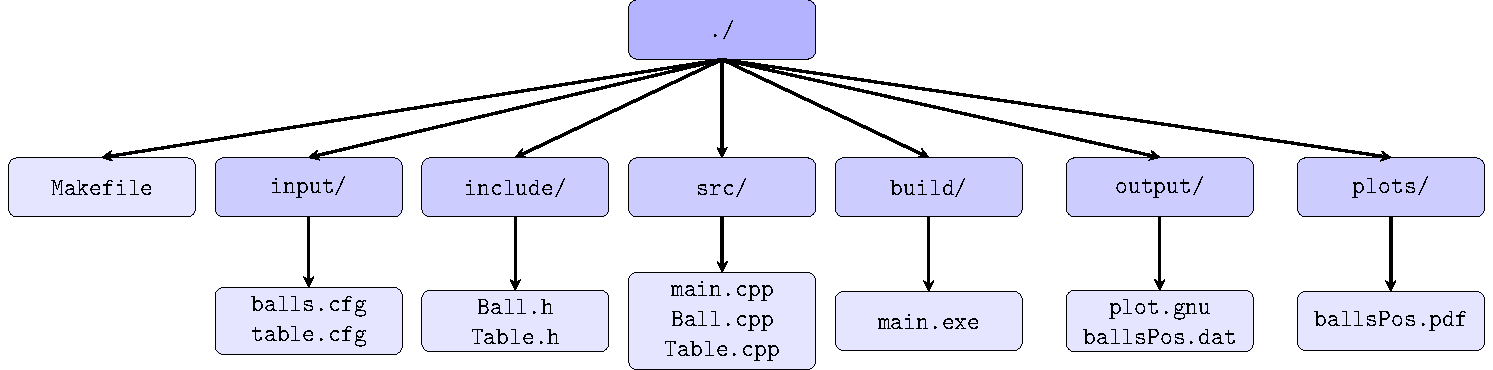
\includegraphics[keepaspectratio, width=1\linewidth]{SchemaArborescence.pdf}
\end{center}

On présente maintenant le contenu de chaque répertoire.

\subsection{Répertoire principal du projet \texttt{./}}

\begin{itemize}
    \myitem \texttt{Makefile}: le fichier à exécuter via la commande \texttt{make} pour compiler le projet;
    \myitem les sous-répertoires décrits plus bas.
\end{itemize}

\subsection{input}

\begin{itemize}
    \myitem \texttt{table.cfg}: fichier de configuration contenant les dimensions de la table de billard ainsi que l'intervalle temporel et le pas temporel;
    \myitem \texttt{balls.cfg}: fichier de configuation contenant les caractéristiques des différentes boules de billard à placer sur la table.
\end{itemize}

\subsection{include}

\begin{itemize}
    \myitem \texttt{Ball.h}: définition de la classe \texttt{Ball}, des ses attributs et des prototypes de ses méthodes;
    \myitem \texttt{Table.h}: définition de la classe \texttt{Table}, des ses attributs et des prototypes de ses méthodes.
\end{itemize}

\subsection{src}

\begin{itemize}
    \myitem \texttt{main.cpp}: le programme principal;
    \myitem \texttt{Ball.cpp}: définition des méthodes de la classe \texttt{Ball};
    \myitem \texttt{Table.cpp}: définition des méthodes de la classe \texttt{Table}.
\end{itemize}

\subsection{build}

\begin{itemize}
    \myitem \texttt{main.exe}: le fichier exécutable produit suite à la compilation du projet.
\end{itemize}

\subsection{output}

\begin{itemize}
    \myitem \texttt{plot.gnu}: fichier de configuration à exécuter via la commande \texttt{gnuplot plot.gnu}. Ce fichier est généré lors de l'exécution du \texttt{main.exe};
    \myitem \texttt{ballsPos.dat}: fichier contenant les positions $(x,y)$ de chaque boule sur la table de billard. Chaque ligne correspond à un instant. Ce fichier est généré lors de l'exécution du \texttt{main.exe} et est appelé dans le script Gnuplot \texttt{plot.gnu}.
\end{itemize}

\subsection{plots}

\begin{itemize}
    \myitem \texttt{ballsPos.pdf}: représentation des trajectoires de boules de billard. Ce fichier est généré par le script \texttt{./output/plot.gnu}.
\end{itemize}

\section{Instructions}

    \subsection{Compilation}

Il faut se placer dans le répertoire principal du projet \texttt{./} puis exécuter le \texttt{Makefile}:
\begin{verbatim}
    cd ./
    make  # ou make -f Makefile
\end{verbatim}
Cela produit le fichier exécutable \texttt{./main/main.exe}.

    \subsection{Exécution}

Se placer dans le répertoire \texttt{./build/} puis exécuter le fichier \texttt{main.exe}:
\begin{verbatim}
    cd ./build/
    ./main.exe
\end{verbatim}
Cela produit les fichiers dans le répertoire \texttt{./output/}

    \subsection{Représentation graphique}

Se placer dans le répertoire \texttt{./output/} puis exécuter le script Gnuplot:
\begin{verbatim}
    cd ./output/
    gnuplot plot.gnu
\end{verbatim}

Cela produit le fichier \texttt{./plots/ballsPos.pdf}.

\end{document}
